\section{Physics Beyond the Standard Model}%
\label{sec:bsm}

The SM is among the most precisely tested theories of physics. It had numerous
successes in predicting phenomena before they were experimentally observed. For
example, the SM predicted the existence of gluons, the $W^\pm$ and $Z$ bosons,
and the Higgs boson prior to their discovery.
% Most recently, the Higgs boson was discovered in 2012 about five decades after
% the inclusion of the BEH mechanism into the SM by Weinberg in
% 1967~\cite{Weinberg:1967tq}. Similarly, the gluons, $W^\pm$ and $Z$ bosons
% were all predicted by the SM before direct experimental evidence for their
% existence could be obtained.
Despite its many successes, the SM is known to be an incomplete theory leaving a
number of phenomena unexplained:
\begin{description}

\item[Matter--antimatter asymmetry] In current cosmological models, equal amounts
  of matter and antimatter are produced in the initial phase of the evolution of
  the universe. However, the universe observed today mostly consists of matter
  particles. This fact is referred to as the matter-antimatter asymmetry of the
  universe. According to the conditions proposed by
  Sakharov~\cite{Sakharov:1967dj}, violation of CP symmetry is required for the
  generation of such an asymmetry in the early universe. While CP violation has
  been observed in the quark sector~\cite{Christenson:1964fg} and first
  indications of CP violation in the lepton sector exist~\cite{T2K:2019bcf}, its
  size might not be sufficient to explain the observed asymmetry.

\item[Gravitation] The theory of general relativity provides an accurate
  description of gravitation in the context of a classical field
  theory. However, no generally accepted approach exists that reconciles general
  relativity with the quantum theory underlying our current formulation of the
  SM. Moreover, understanding the weakness of gravitational interactions at the
  scale of elementary particles remains one of the open questions in particle
  physics.

\item[Dark matter] Astrophysical
  observations~\cite{Zwicky:1933gu,Zwicky:1937zza,Rubin:1970zza,Rubin:1980zd,Clowe:2006eq}
  indicate that the vast majority of the universe consists of a form of matter,
  referred to as \emph{dark matter}, that does not interact via the
  electromagnetic interaction. However, its existence can be inferred from the
  gravitational interaction between dark and ordinary matter. Provided dark
  matter is microscopic in nature, the SM does not provide a suitable dark
  matter candidate that is consistent with current cosmological models.

\item[The electroweak hierarchy problem] The mass of the Higgs boson is affected
  by virtual corrections involving loops of massive particles. These corrections
  diverge quadratically with the momentum scale $\Lambda$~\cite{Giudice:2008bi},
  which is the upper cut-off of the loop momentum integration. Based on
  arguments of
  \emph{naturalness}~\cite{Gildener:1976ai,Weinberg:1978ym,Susskind:1978ms,Giudice:2008bi},
  the radiative corrections to the Higgs boson mass should not exceed the
  electroweak scale of $\mathcal{O}(\SI{100}{\GeV})$. Under this assumption, the
  SM cannot remain valid beyond a scale of $\mathcal{O}(\SI{1}{\TeV})$, at which
  point the divergences would have to be regulated by BSM physics
  contributions. At the LHC, the SM is being probed at this scale and beyond,
  however, no direct signs of new physics have been observed thus
  far. Consequently, it needs to be considered that the SM remains valid up to a
  larger energy scale, for example the scale of a \emph{Grand Unified Theory}
  (GUT) of about $10^{16}\,\si{\GeV}$~\cite{pdg2020}. In this case, for the
  Higgs boson mass to remain at the electroweak scale would require excessive
  \emph{fine-tuning} of the theory parameters, otherwise radiative corrections
  would drag the Higgs boson mass towards, for example, the GUT scale.

\item[Neutrino masses] The observation of neutrino
  oscillations~\cite{Super-Kamiokande:1998kpq,SNO:2002tuh} constitutes
  experimental evidence of neutrinos being massive particles. In the SM, it is
  assumed that neutrinos are massless particles, however. Extending the SM to
  incorporate non-vanishing neutrino masses poses the question whether neutrinos
  are Dirac or Majorana~\cite{Majorana:1937vz} particles. In addition, upper
  limits on the neutrino masses are $\mathcal{O}(\SI{1}{\electronvolt})$ for
  electron-based measurements~\cite{KATRIN:2019yun}, which
  % , adopting arguments of \emph{naturalness},
  appear to be unnaturally small compared to the mass scales of other fermions
  (\SI{1}{\MeV} to \SI{100}{\GeV}).

  % If neutrinos are Dirac particles, then a
  % Dirac mass term can be introduced into the SM Lagrangian via Yukawa
  % interactions between neutrinos and the Higgs boson. This mass term couples
  % left- and right-handed neutrino chiral states, implying the existence of a
  % non-interacting (\emph{sterile}) degree of freedom.

  % If neutrinos are Dirac particles, then the
  % addition of a Dirac mass term into the SM Lagrangian introduces a coupling
  % between left- and right-handed neutrino chiral states. This implies the
  % existence of a non-interacting (\emph{sterile}) degree of freedom for
  % neutrinos, since right-handed neutrinos (left-handed anti-neutrinos) do not
  % participate in the weak interaction. While the neutrino masses could be
  % generated via Yukawa couplings to the Higgs field, the coupling strengths
  % differ by many orders of magnitude compared to other fermions. The alternative
  % hypothesis of neutrinos being Majorana particles~\cite{Majorana:1937vz}, i.e.\
  % neutrinos are their own anti-particles,

  % - lepton number violation (neutrinoless double-$\beta$ decay)

  % \emph{see-saw mechanism}

  % Majorana:
  % - Neutrinos and antineutrinos are the same particle
  % - No sterile neutrinos
  % - Seesaw mechanism could explain the small mass of neutrinos

% Is this really a 'problem'?
% \item[Vacuum Stability] The present minimum with a vacuum expectation value of
%   $\varv \approx \si{246}{\GeV}$ might be either a global minimum in which case the
%   universe is stable or only a local minimum which leads to a metastable
%   universe. In the metastable case, the state of the Higgs field could tunnel to
%   a new local or global minimum with a smaller potential. Current experimental
%   data cannot distinguish whether the universe is stable or
%   meta-stable\todo{citation}.

\end{description}
Even though the SM has its shortcomings, it describes many natural phenomena
with excellent precision. Thus, it is often believed that the SM represents the
low-energy manifestation of an extended theory that only becomes relevant at
larger energy scales, for example a \emph{Grand Unified Theory} that unifies the
electroweak and strong interaction.


\subsection{Non-Resonant Higgs Boson Pair Production}%
\label{sec:bsm_nonresonant_hh}

BSM phenomena might appear at energy scales beyond what can be experimentally
probed using direct searches\footnote{i.e.\ searches for on-shell production of
  BSM particles.} at the LHC. Nevertheless, it is possible to test such models
indirectly through their contributions to SM processes via virtual
corrections. These corrections can, for example, alter the total or differential
cross section of a given process.
% Therefore, searches for non-resonant \HH production are already of interest,
% since an enhancement in its cross section would be indicative of BSM physics.

% Another way...
A way of exploring BSM contributions to non-resonant \HH production is to
examine the Higgs boson self-coupling constant for possible deviations from the
SM value of $\lambda_{HHH}^\text{SM} = 3 m_{H}^2 / \varv$. Such deviations can
arise due to virtual corrections involving massive BSM particles as indicated in
\Cref{fig:bsm_hh_prod_feyn}. If the mass scale of the particles participating in
the corrections is sufficiently large, then the dynamics of the BSM theory can
be reduced to an effective interaction vertex between three Higgs bosons with a
coupling constant
\begin{align*}
  \lambda_{HHH} = \klambda \times \lambda_{HHH}^{\text{SM}} \,\text{,}
\end{align*}
where \klambda is an arbitrary coupling modifier. A change in \klambda would
alter both the total cross section of non-resonant \HH production and the
kinematics of the final state particles. These effects are discussed in
\Cref{sec:higgs_self_coupling}.

\begin{figure}[htbp]
  \centering

  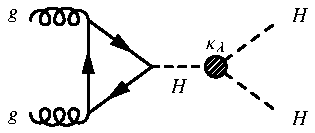
\includegraphics[width=0.35\textwidth]{feynman_graphs/di_higgs_effective}

  \caption[Feynman diagram of non-resonant \HH production with anomalous values
  of the Higgs boson self-coupling.]{Non-resonant production of Higgs boson
    pairs for anomalous values of the Higgs boson self-coupling constant.
    Contributions of new physics, for example through loops of heavy BSM
    particles, are indicated as a hatched circle. The effective coupling
    constant in units of the self-coupling constant predicted by the SM is given
    by \klambda.}%
  \label{fig:bsm_hh_prod_feyn}
\end{figure}

% Unitarity: Scattering probability < 1
%
% Perturbativity: Higher-order corrections become smaller as opposed to larger
Current bounds on possible values of \klambda from requirements of perturbative
unitarity in $HH \to HH$ scattering allow for variations within
$|\klambda| \lessapprox 6$~\cite{DiLuzio:2017tfn}.\footnote{Similar arguments
  were made in the past to obtain upper limits on the Higgs boson mass from
  unitarity bounds in the scattering of longitudinally polarised vector
  bosons~\cite{Lee:1977eg}.} These bounds still allow for ample variation of the
Higgs boson self-coupling strength, further motivating searches for non-resonant
\HH production. These searches constitute a major part of
\Cref{sec:dihiggs,sec:higgs_self_coupling} in which upper limits are set on the
non-resonant \HH production cross section of a signal with SM-like
($\klambda = 1$) kinematics, and signals with anomalous \klambda
($\klambda \neq 1$), respectively.

% Anomalous values of the Higgs boson self-coupling within
% $|\klambda| \lessapprox 6$ are allowed given arguments based on the unitarity
% and perturbativity of $HH \to HH$
% scattering~\cite{DiLuzio:2017tfn}.\footnote{Similar arguments were made in the
%   past to obtain upper limits on the Higgs boson mass from unitarity bounds in
%   the scattering of longitudinally polarised vector bosons~\cite{Lee:1977eg}.}


\subsection{Resonant Higgs Boson Pair Production}%
\label{sec:bsm_resonant_hh}

If BSM physics occurs at experimentally accessible energy scales, new particles
could be produced directly (on-shell) in collider experiments. Further assuming
that these particles are short-lived and decay into detectable SM particles, one
can reconstruct the mass of such particles using the four-momenta of their decay
products. The presence of BSM physics can then appear as an enhancement of the
differential cross section $\mathrm{d}\sigma / \mathrm{d}m$, $m$ referring to
the invariant mass of the final state particles, in a region close to the mass
of the new particle. This phenomenon is referred to as a \emph{resonance} and
the production of particles via an intermediate resonance as \emph{resonant
  production}.

The Higgs sector is often used as an entry point for physics beyond the
SM. Aside from aesthetic reasons, there are currently no arguments that require
nature to realise a \emph{minimal Higgs model} with a single
Higgs-doublet~\cite{Gunion:1989we}. In fact, the Higgs sector can be readily
extended with additional scalar fields with singlet and doublet representations
under the SM gauge group~\cite{Gunion:1989we}. Such extended Higgs sectors are
part of many BSM theories, resulting in a phenomenology with new scalar
particles. Under certain circumstances, these models allow for a sizeable
production of SM-like Higgs boson pairs via intermediate scalar resonances. A
possible Feynman diagram of resonant Higgs boson pair production is depicted in
\Cref{fig:resonant_production_feyn}. Two examples of models with extended Higgs
sectors are given in the following.

\begin{figure}[htbp]
  \centering

  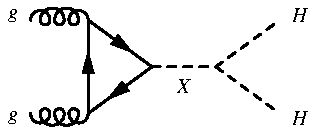
\includegraphics[width=0.35\textwidth]{feynman_graphs/di_higgs_resonant}

  \caption[Feynman diagram of resonant Higgs boson pair production.]{Resonant
    production of SM Higgs boson pairs via an intermediate scalar resonance $X$
    produced in \ggF.}%
  \label{fig:resonant_production_feyn}
\end{figure}

\begin{description}

\item[Additional Higgs-singlet models] The simplest extension of the SM Higgs
  sector is the addition of a real scalar field $\phi_{S}$ that transforms as a
  singlet under the SM gauge group. This scalar field, being a gauge singlet,
  does not interact with any of the SM fermions or vector bosons. It could
  therefore be part of a ``hidden sector'' which might provide a suitable
  candidate for dark matter. In so-called \emph{Higgs portal
    models}~\cite{Patt:2006fw}, the hidden sector can only be accessed through
  coupling/mixing of $\phi_{S}$ with the CP-even component of the SM Higgs
  field. Such models can predict resonant production of Higgs boson pairs
  through new scalar
  resonances~\cite{Schabinger:2005ei,Bowen:2007ia,Barger:2007im,Dolan:2012ac,No:2013wsa,Chen:2014ask,Robens:2016xkb,DiMicco:2019ngk}.

  A general choice for the potential of a Higgs sector extended by an additional
  scalar field
  reads~\cite{OConnell:2006rsp,No:2013wsa,Chen:2014ask,DiMicco:2019ngk}
  \begin{align*}
    V(\phi, \phi_{S}) = V(\phi)
    + \frac{a_1}{2} (\phi^\dagger \phi) \phi_{S}
    + \frac{a_2}{2} (\phi^\dagger \phi) \phi_{S}^2
    + b_1 \phi_{S} + \frac{b_2}{2} \phi_{S}^2 + \frac{b_3}{3} \phi_{S}^3 + \frac{b_4}{4} \phi_{S}^4 \,\text{,}
  \end{align*}
  where $\phi$ refers to the complex Higgs-doublet and $V(\phi)$ is the BEH
  potential. In unitary gauge, the fields can be expanded about the vacuum state
  as $\phi = (0, \varv + H)^{\text{T}} / \sqrt{2}$ and $\phi_{S} = \varv_{S} + S$, where
  $\varv_{S}$ is the VEV of $\phi_{S}$. After the expansion, terms bilinear in $H$
  and $S$ appear in the potential,\footnote{The bilinear terms only appear if
    either $a_1 \neq 0$, or $a_2 \neq 0$ and $\phi_{S}$ has non-vanishing
    VEV. See for example Ref.~\cite{Chen:2014ask}.} which indicate that the
  physical fields are mixtures of $H$ and $S$. The physical fields $H_1$ and
  $H_2$ with masses $m_1$ and $m_2$, respectively, can be expressed as
  \begin{align*}
    \begin{pmatrix}
      H_1 \\
      H_2
    \end{pmatrix}
    =
    \begin{pmatrix}
      \cos\theta & \sin\theta \\
      -\sin\theta & \cos\theta
    \end{pmatrix}
    \begin{pmatrix}
      H \\
      S
    \end{pmatrix} \,\text{,}
  \end{align*}
  with a mixing angle $\theta$. In the following, it is assumed that $H_1$ can
  be identified with the observed Higgs boson and $H_2$ is a new scalar with
  $m_2 > 2 m_1$.  The scalar $H_2$ can be produced via \ggF through the
  admixture of $H$ in $H_2$, however, suppressed by a factor of
  $\sin^2\theta$. Further, the interaction terms of the scalar potential allow
  for decays of $H_2$ into a pair of $H_1$. As a consequence, resonant
  production processes according to $\pp \to H_2 \to H_1 H_1$ are possible given
  the prior assumptions.

\item[Two-Higgs-doublet models (2HDM)] Generic 2HDM extend the Higgs sector of
  the SM by introducing an additional $SU(2)_{\text{L}}$ doublet of complex
  scalar fields~\cite{Gunion:1989we,Branco:2011iw}. Such extensions are
  motivated by theories such as supersymmetry~\cite{Haber:1984rc}, which require
  at least two Higgs-doublets to generate masses of up- ($I_3 = + 1/2$) and
  down-type ($I_3 = - 1/2$) fermions, or models of electroweak
  baryogenesis~\cite{Trodden:1998ym} in which 2HDM can provide CP-violating
  processes necessary to generate a matter-antimatter asymmetry in the universe.
  % The class of 2HDM encompass theories with vastly different phenomenology.
  % For example, 2HDM with flavour-changing neutral currents (FCNC) at
  % tree-level exist, however, such models are in tension with the experimental
  % non-observation of tree-level FCNC~\cite{Gunion:1989we,Branco:2011iw}.

  Further discussion is restricted to flavour- and CP-conserving 2HDM, which,
  for example, include models describing the Higgs sector of minimal
  supersymmetric extensions of the SM (MSSM).\footnote{For CP-violating 2HDM as
    possible explanations of electroweak baryogenesis, see for example the
    \emph{complex 2HDM} (C2HDM) in Ref.~\cite{Fontes:2017zfn}.}
  % The Higgs doublets in 2HDM have non-vanishing VEV denoted $\varv_1$ and $\varv_2$,
  % respectively.  , often expressed as the ratio
  % $\tan\beta \coloneqq \varv_2 / \varv_1$.
  The particle spectrum of these models consist of five scalar particles after
  EWSB: two CP-even Higgs bosons $H_1$ and $H_2$, a CP-odd Higgs boson $A$, and
  two charged Higgs bosons $H^\pm$. Similar to the model with an additional
  Higgs-singlet, the physical fields $H_1$ and $H_2$ are mixed states of the
  CP-even components of both Higgs-doublets, and interaction vertices of the
  form $H_1 H_1 H_2$ exist~\cite{Gunion:1989we,Branco:2011iw}. This can allow
  for resonant production processes according to $\pp \to H_2 \to H_1 H_1$,
  which are promising search channel for heavy, CP-even Higgs boson in certain
  BSM scenarios~\cite{Dolan:2012ac,Djouadi:2013vqa,Djouadi:2013uqa}.

\end{description}
The selected examples are not intended to be comprehensive but rather serve to
illustrate how resonant \HH production can arise in models with extended Higgs
sectors. In this thesis, the benchmark signal process is the decay of a CP-even
scalar resonance, $X$, produced via \ggF into a pair of SM Higgs bosons as
depicted in \Cref{fig:resonant_production_feyn}. The width of the resonance is
assumed to be narrow such that interference with SM \HH production can be
neglected.

%%% Local Variables:
%%% mode: latex
%%% TeX-master: "../../phd_thesis"
%%% End:
